\documentclass{beamer}

\usetheme{McMaster}
\usepackage{math}
\usepackage{tikz, pgfplots}
\usepackage{tikz-3dplot}
\usetikzlibrary{decorations.pathreplacing,positioning,calc,intersections,3d,shapes.geometric,shapes,chains,math,fit,backgrounds}


\begin{document}

% Schwarz (incl. keyhole domain)
\begin{frame}{H.A. Schwarz, 1869}

How do we solve the Laplace equation on complicated domains?

We split the domain into simpler subdomains.

\begin{figure}
	\centering
	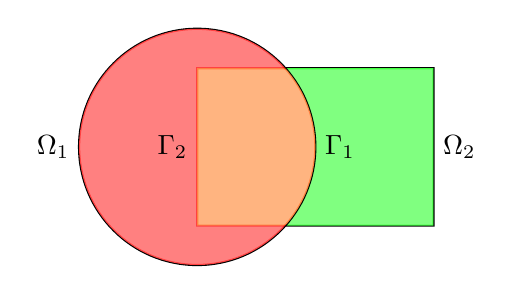
\begin{tikzpicture}
		\begin{scope}[blend group = soft light]
			\filldraw[draw=black, fill=red!50!white, thick] (0,0) circle (1.5);
			\filldraw[draw=black, fill=green!50!white, thick] (0,-1) rectangle (3,1);
		\end{scope}
		\node[left] at (-1.5,0) {$\Omega_1$};
		\node[right] at (3,0) {$\Omega_2$};
		\node[left] at (0,0) {$\Gamma_2$};
		\node[right] at (1.5,0) {$\Gamma_1$};
	\end{tikzpicture}
%\vspace{-3em}
%\includegraphics[width=0.5\textwidth]{AOSM/FIG_keyhole.png}
%\vspace{-4em}
%\caption{Schwarz's original example, taken from wikimedia.org}
\end{figure}

Alternating Schwarz method:
\begin{equation*}
	\begin{cases} \Delta u_1^{n+1} = 0 & \text{in } \Omega_1, \\ u_1^{n+1} = u_2^n & \text{on } \Gamma_1, \end{cases}
	\quad
	\begin{cases} \Delta u_2^{n+1} = 0 & \text{in } \Omega_2, \\ u_2^{n+1} = u_1^{n+1} & \text{on } \Gamma_2. \end{cases}
\end{equation*}
\end{frame}

\begin{frame}{Algebraic decomposition}

The subproblem on $\Omega_1$ is
\begin{equation*}
		\begin{bmatrix} A_{11} & A_{1 \Gamma} \\ A_{\Gamma 1} & A_{\Gamma \Gamma} + T_{2 \to 1} \end{bmatrix}
                            \begin{bmatrix} \vec{u}_1^{n+1} \\ \vec{u}_{1 \Gamma}^{n+1} \end{bmatrix}
                            = \begin{bmatrix} \vec{f}_1 \\ \vec{f}_\Gamma \end{bmatrix}
                            + \begin{bmatrix} ~ \\ -A_{\Gamma 2} \vec{u}_2^n + T_{2 \to 1} \vec{u}_{2 \Gamma}^n \end{bmatrix}
\end{equation*}
and the subproblem on $\Omega_2$ is
\begin{equation*}
       \begin{bmatrix} A_{22} & A_{2 \Gamma} \\ A_{\Gamma 2} & A_{\Gamma \Gamma} + T_{1 \to 2} \end{bmatrix}
                            \begin{bmatrix} \vec{u}_2^{n+1} \\ \vec{u}_{2 \Gamma}^{n+1} \end{bmatrix}
                            = \begin{bmatrix} \vec{f}_2 \\ \vec{f}_\Gamma \end{bmatrix}
                            + \begin{bmatrix} ~ \\ -A_{\Gamma 1} \vec{u}_1^n + T_{1 \to 2} \vec{u}_{1 \Gamma}^n \end{bmatrix}.
\end{equation*}

$\vec{u}_\Gamma$ appears in both subproblems since the interface is shared between the two subdomains.
These copies are distinct and must be recombined in some way at the end, for example:
\begin{equation*}
	\vec{u}_\Gamma = \frac{\vec{u}_{1 \Gamma} + \vec{u}_{2 \Gamma} }{2}.
\end{equation*}
\end{frame}

\begin{frame}
\frametitle{What is a symmetrized cell?}

\begin{columns}
	\begin{column}{0.5\textwidth}
For each subdomain, take a copy of it and stitch it together along their shared interface.
This pair is now perfectly symmetric, and one subproblem describes both copies.
	\end{column}

\tdplotsetmaincoords{60}{110}
\def\SplitAngle{120}
\def\AngleSplit{300}
	\begin{column}{0.5\textwidth}
\begin{figure}
	\begin{tikzpicture}[tdplot_main_coords]
		\fill[left color=blue!50] (180:1 and 1) arc (180:\AngleSplit:1 and 1) -- ++(0,0,2) arc (\AngleSplit:180:1 and 1) -- cycle;
		\fill[left color=blue!50] (1,0,0) arc (360:\AngleSplit:1 and 1) -- ++(0,0,2) arc (\AngleSplit:360:1 and 1) -- cycle;
		\foreach \x in {-2,...,2} {
			\draw[gray, thin] (\x,0,-1) -- (\x,0,3);
		}
		\foreach \z in {-1,...,3} {
			\draw[gray, thin] (-2,0,\z) -- (2,0,\z);
		}
		\fill[right color=red!10] (\SplitAngle:1 and 1) arc (\SplitAngle:180:1 and 1) -- ++(0,0,2) arc (180:\SplitAngle:1 and 1) -- cycle;
		\fill[right color=red!10] (1,0,0) arc (0:\SplitAngle:1 and 1) -- ++(0,0,2) arc (\SplitAngle:0:1 and 1) -- cycle;
	\end{tikzpicture}
	\caption{A symmetrized square domain with interfaces on two opposing edges}
\end{figure}
	\end{column}
\end{columns}
\end{frame}


\end{document}